\documentclass{beamer}
\usepackage{amsmath}
\usepackage{hyperref}
\usepackage{graphicx}
\usepackage{tikz}
\addtobeamertemplate{frametitle}{}{%
    \begin{tikzpicture}[remember picture,overlay]
        \node[anchor=north east, xshift=-0.5cm, yshift=-0.1cm] at (current page.north east) {
            
\includegraphics[width=1.5cm]{imgs/kth-logo.png}
        };
    \end{tikzpicture}
}

\title{Lecture: Data Analysis and Machine Learning Theory}
\author{KTH AI Student}
\date{\today}

\begin{document}

\frame{\titlepage}

\section{About me}
\begin{frame}{About me}
\begin{itemize}
    \item Jag heter Martín! I am from Chile, did my Bachelor's Degree at Universidad de Chile, doing a year-long exchange at KTH.
    \item I am currently interning at Hopsworks, an AI Lakehouse in Stockholm. Working on ML pipelines and LLMs.
    \item I enjoy running, hiking, and trying to improve my awful Swedish.
\end{itemize}
\begin{figure}
    \centering
    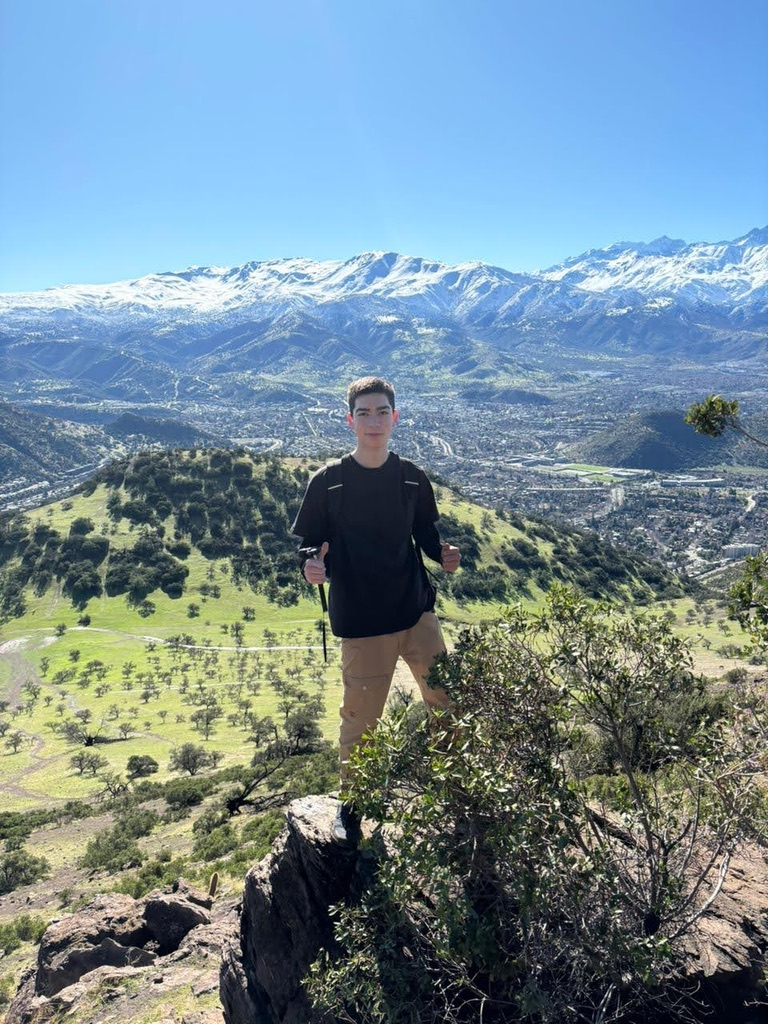
\includegraphics[width=4cm]{imgs/me.jpeg}
    
\includegraphics[width=5cm]{imgs/empire.png}
\end{figure}
\end{frame}

\begin{frame}{In this lecture}
    \begin{itemize}
        \item We will review key concepts in data analysis and machine learning theory.
        \begin{itemize}
            \item Descriptive Statistics and Data Visualization.
            \item Probability Theory and Simulation.
            \item Correlation and Regression Analysis.
            \item A/B Testing and Hypothesis Testing.
        \end{itemize}
    \end{itemize}
    \end{frame}
    

\section{Descriptive Statistics and Data Visualization}

\begin{frame}{Question 1}
    Imagine we have a big dataset, and we want to summarize it. What are some ways we can do this?
    \end{frame}
\begin{frame}{Example: Student Test Scores}
    \begin{itemize}
        \item \textbf{Dataset:} Contains scores of students.
        \item \textbf{Goals:}
        \begin{itemize}
            \item Compute key descriptive statistics to summarize performance.
            \item Visualize score distributions to identify trends or outliers.
            \item Provide actionable insights to improve teaching methods.
        \end{itemize}
    \end{itemize}
    \end{frame}

\begin{frame}{Key Concepts}
\textbf{Descriptive Statistics:} Summarize and describe the main features of a dataset.
\begin{itemize}
    \item \textbf{Mean}: The average value of a dataset.
    $$ \bar{x} = \frac{1}{n} \sum_{i=1}^{n} x_i $$
    \item \textbf{Median}: The middle value when data is sorted.
    $$ x_{\text{median}} = \begin{cases} x_{(n+1)/2} & \text{if } n \text{ is odd} \\ \frac{1}{2} (x_{n/2} + x_{n/2+1}) & \text{if } n \text{ is even} \end{cases} $$
    \item \textbf{Mode}: The most frequently occurring value.
    $$ x_{\text{mode}} = \text{value with highest frequency} $$
\end{itemize}
\end{frame}

\begin{frame}{Key Concepts}
\begin{itemize}
    \item \textbf{Variance}: Measures the spread of data points from the mean.
    $$ \sigma^2 = \frac{1}{n} \sum_{i=1}^{n} (x_i - \bar{x})^2 $$
    \item \textbf{Standard Deviation}: Square root of variance, represents data dispersion.
    $$ \text{SD} = \sqrt{\sigma^2} $$
    \item \textbf{Range}: Difference between the maximum and minimum values.
    $$ \text{Range} = \max(x) - \min(x) $$
\end{itemize}
\end{frame}


\begin{frame}{Key Concepts}
\textbf{Data Visualization:} Graphical representation of data.
\begin{itemize}
    \item \textbf{Histograms}: Show frequency distribution of data.
        \begin{figure}
            \centering
            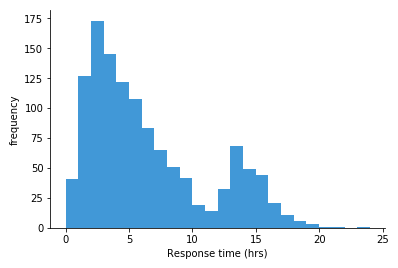
\includegraphics[width=0.5\textwidth]{imgs/histogram.png}
        \end{figure}
    \item \textbf{Box Plots}: Visualize data spread and identify outliers.
        \begin{figure}
            \centering
            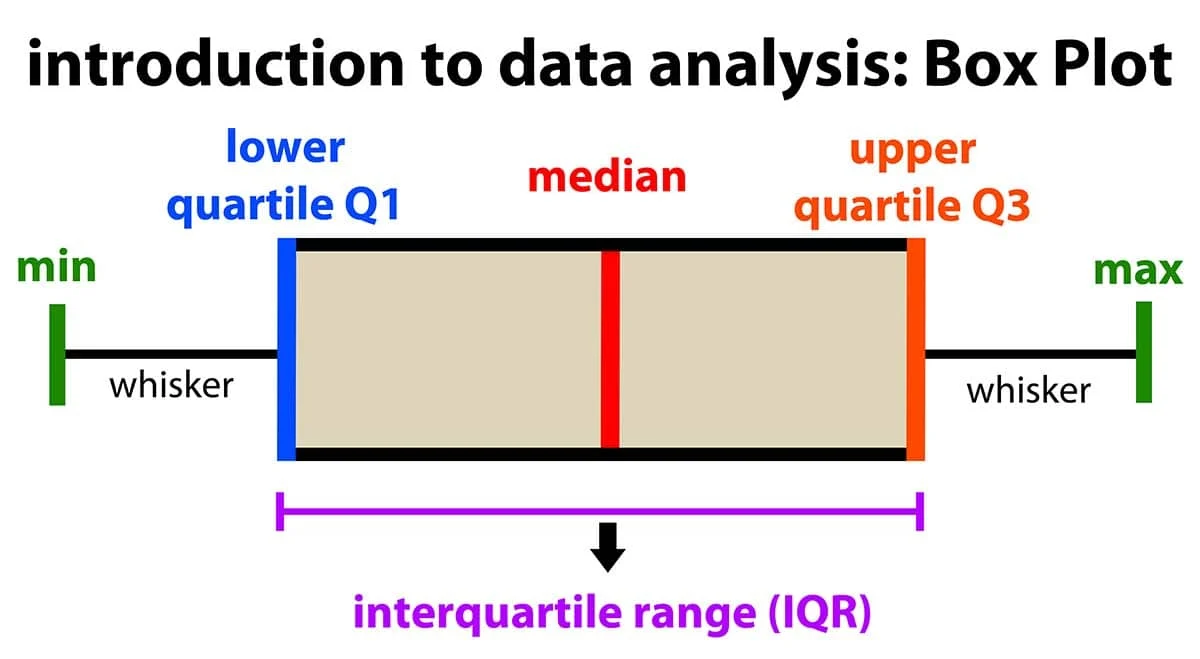
\includegraphics[width=0.5\textwidth]{imgs/box-plot.png}
        \end{figure}
    \end{itemize}
\end{frame}

\begin{frame}{Key Concepts}
\begin{itemize}
    \item \textbf{Scatter Plots}: Display relationships between two variables.
    \begin{figure}
        \centering
        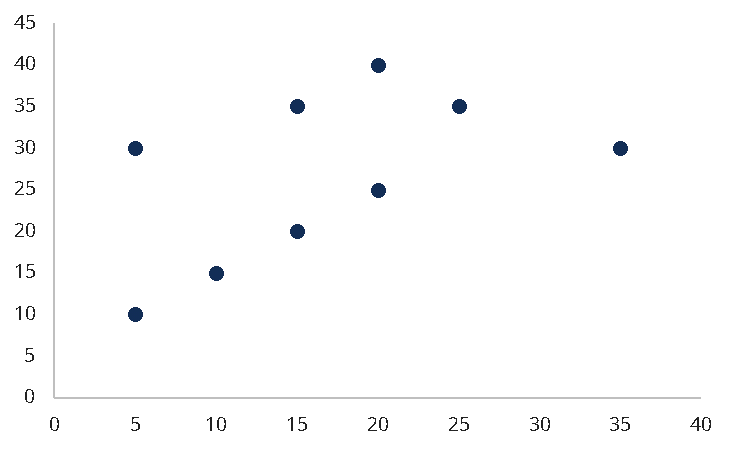
\includegraphics[width=0.5\textwidth]{imgs/scatter-plot.png}
    \end{figure}
    \item \textbf{Bar Charts}: Compare categorical data.
    \begin{figure}
        \centering
        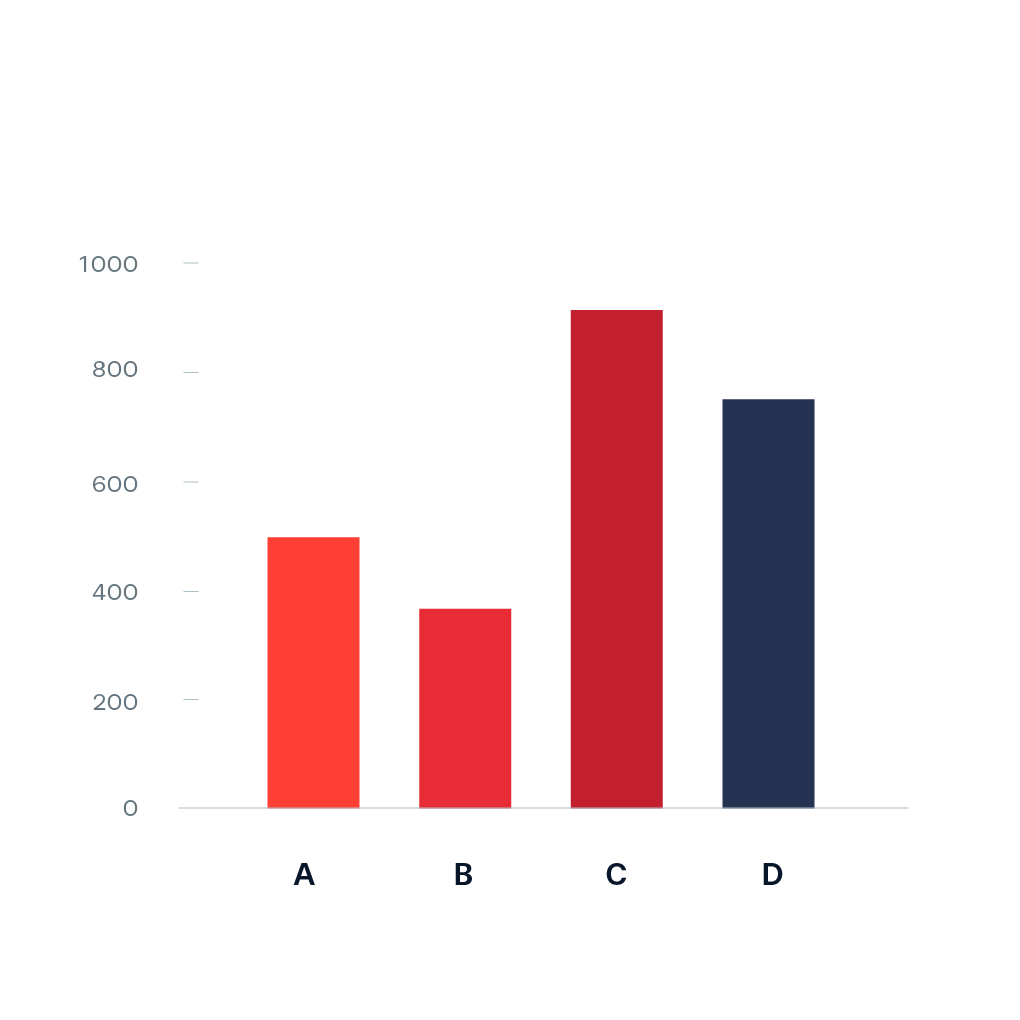
\includegraphics[width=0.3\textwidth]{imgs/bar-chart.png}
    \end{figure}
\end{itemize}
\end{frame}


\section{Probability Theory and Simulation}

\begin{frame}{Question 2}
    We have a dataset, but does this dataset represent the real world? How can we estimate the probability of events?
\end{frame}


\begin{frame}{Example: Simulation Tasks}
    \begin{itemize}
        \item Simulate 1000 coin tosses to calculate the probability of heads and compare with theoretical value.
        \item Simulate 1000 dice rolls to calculate:
        \begin{itemize}
            \item Probability of rolling a prime number.
            \item Conditional probability of a prime given the number is odd.
        \end{itemize}
        \item Use Monte Carlo simulation to estimate $\pi$.
    \end{itemize}
    \end{frame}


\begin{frame}{Key Concepts: Probability}
\begin{itemize}
    \item \textbf{Probability:} Study of the likelihood of events.
    \begin{itemize}
        \item \textbf{Theoretical Probability:} Based on known outcomes (e.g., coin toss).
        $$ P(A) = \frac{\text{Number of favorable outcomes}}{\text{Total number of outcomes}} $$
        \item \textbf{Simulated Probability:} Estimated by running experiments or simulations.
        \item \textbf{Bayes' Theorem:} Describes conditional probability, updates beliefs based on evidence.
        $$ P(A|B) = \frac{P(B|A) \cdot P(A)}{P(B)} $$
    \end{itemize}
\end{itemize}
\end{frame}

\begin{frame}{Key Concepts: Probability Distributions}
\begin{itemize}
    \item \textbf{Probability Distributions:} Represent how probabilities are distributed over values.
    \begin{itemize}
        \item \textbf{Uniform Distribution:} All outcomes are equally likely.
        $$ P(x) = \frac{1}{n} \quad \text{for } x \in \{1, 2, \ldots, n\} $$
        \item \textbf{Binomial Distribution:} Number of successes in fixed trials.
        $$ P(X = k) = \binom{n}{k} p^k (1-p)^{n-k} $$
        \item \textbf{Normal Distribution:} Bell-shaped curve, common in natural data.
        $$ f(x) = \frac{1}{\sqrt{2\pi\sigma^2}} e^{-\frac{(x-\mu)^2}{2\sigma^2}} $$
    \end{itemize}
\end{itemize}
\end{frame}

\begin{frame}{Key Concepts: Monte Carlo Simulation}
\begin{itemize}
    \item \textbf{Monte Carlo Simulation:} Uses random sampling to estimate mathematical results.
    \begin{itemize}
        \item Example: Estimate $\pi$ by generating random points in a square and calculating the ratio inside a quarter circle.
        $$ \pi \approx 4 \times \frac{\text{Number of points inside circle}}{\text{Total number of points}} $$
    \end{itemize}
\end{itemize}
\end{frame}


\section{Correlation and Regression Analysis}

\begin{frame}{Question 3}
    We have two variables, how can we determine if they are related? How can we predict one variable based on the other?
\end{frame}

\begin{frame}{Example: Car Prices and Mileage}
    \begin{itemize}
        \item \textbf{Dataset:} Contains car prices and mileage.
        \item \textbf{Tasks:}
        \begin{itemize}
            \item Compute the correlation coefficient to assess the strength and direction of the relationship.
            \item Build a simple linear regression model to predict prices based on mileage.
            \item Visualize the data and regression line to interpret the results.
        \end{itemize}
    \end{itemize}
\end{frame}
    

\begin{frame}{Key Concepts: Correlation}
\begin{itemize}
    \item \textbf{Correlation:} Measures the strength and direction of the linear relationship between two variables.
    \begin{itemize}
        \item \textbf{Range:} Values range from $-1$ to $1$.
        \item \textbf{Interpretation:}
        \begin{itemize}
            \item $1$: Perfect positive correlation.
            \item $-1$: Perfect negative correlation.
            \item $0$: No linear correlation.
        \end{itemize}
    \end{itemize}
\end{itemize}
\end{frame}

\begin{frame}{Key Concepts: Correlation}
\begin{itemize}
    \item \textbf{Correlation Coefficient:} Denoted by $r$.
    $$ r = \frac{\sum_{i=1}^{n} (x_i - \bar{x})(y_i - \bar{y})}{\sqrt{\sum_{i=1}^{n} (x_i - \bar{x})^2} \sqrt{\sum_{i=1}^{n} (y_i - \bar{y})^2}} $$
    \item \textbf{Correlation Matrix:} Displays pairwise correlations between variables.
\end{itemize}
\begin{figure}
    \centering
    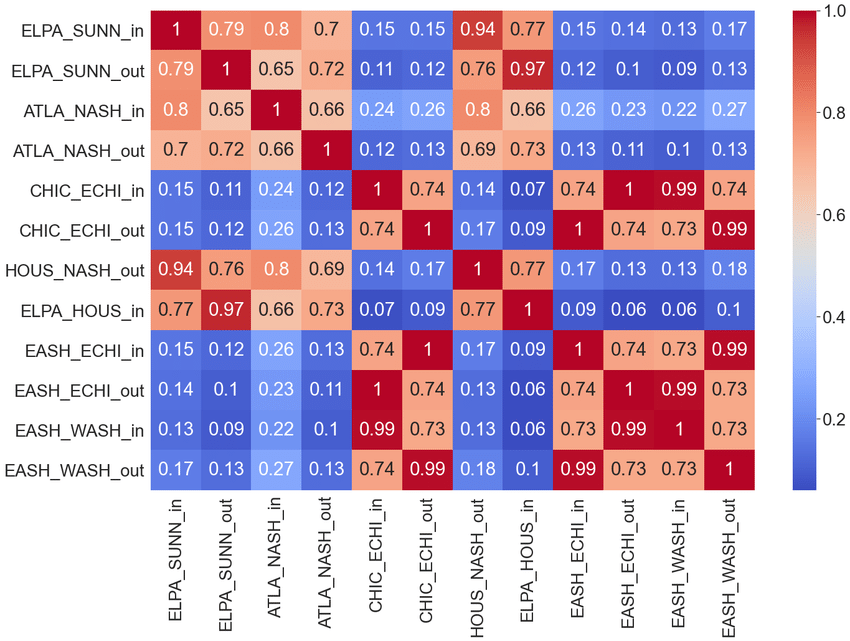
\includegraphics[width=0.5\textwidth]{imgs/correlation.png}
\end{figure}
\end{frame}


\begin{frame}{Key Concepts: Regression Analysis}
\begin{itemize}
    \item \textbf{Regression Analysis:} Models the relationship between a dependent variable and one or more independent variables.
    \begin{itemize}
        \item \textbf{Simple Linear Regression:} $y = \beta_0 + \beta_1 x + \epsilon$
        \item \textbf{Goals:}
        \begin{itemize}
            \item Estimate the coefficients ($\beta_0$, $\beta_1$).
            \item Minimize prediction error ($\epsilon$).
        \end{itemize}
        \item \textbf{Evaluation Metrics:} Assess model fit using metrics such as Mean Squared Error (MSE).
    \end{itemize}
\end{itemize}
\begin{figure}
    \centering
    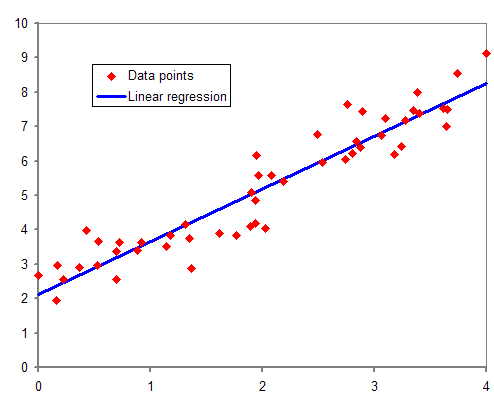
\includegraphics[width=0.5\textwidth]{imgs/regression.png}
\end{figure}
\end{frame}


\section{A/B Testing and Hypothesis Testing}

\begin{frame}{Question 4}
    We have two groups, how can we determine if they are significantly different? How can we validate our assumptions?
\end{frame}


\begin{frame}{Example: Website Redesign A/B Test}
    \begin{itemize}
        \item \textbf{Dataset:} User engagement metrics for old and new designs.
        \item \textbf{Tasks:}
        \begin{itemize}
            \item Perform a t-test to compare engagement levels.
            \item Calculate and interpret the p-value.
            \item Determine whether the new design significantly improves engagement.
        \end{itemize}
    \end{itemize}
    \end{frame}

\begin{frame}{Key Concepts: Hypothesis Testing}

\begin{itemize}
    \item \textbf{Hypothesis Testing:} Framework to evaluate whether observed data provides sufficient evidence to reject a null hypothesis ($H_0$).
    \begin{itemize}
        \item \textbf{Null Hypothesis ($H_0$):} Assumes no effect or difference.
        \item \textbf{Alternative Hypothesis ($H_a$):} Suggests a significant effect or difference.
    \end{itemize}
    \item \textbf{t-Test:} Compares means of two groups.
    \begin{itemize}
        \item \textbf{t-statistic:} Quantifies the difference relative to variability.
        \item \textbf{p-value:} Probability of observing results as extreme as the data, assuming $H_0$ is true.
    \end{itemize}
    \item \textbf{Significance Level:} Common threshold $\alpha = 0.05$.
\end{itemize}
\end{frame}

\begin{frame}{Key Concepts: Hypothesis Testing}
\begin{itemize}
    \item \textbf{Interpretation:}
    \begin{itemize}
        \item \textbf{p-value $< \alpha$:} Reject $H_0$, evidence supports $H_a$.
        \item \textbf{p-value $\geq \alpha$:} Fail to reject $H_0$, insufficient evidence.
    \end{itemize}
    \item \textbf{Type I Error:} Incorrectly reject $H_0$ (false positive).
    \item \textbf{Type II Error:} Incorrectly fail to reject $H_0$ (false negative).
    \item \textbf{Power:} Probability of correctly rejecting $H_0$.
\end{itemize}
\end{frame}

\begin{frame}{Key Concepts: Hypothesis Testing}
How to perform a t-test:
\begin{enumerate}
    \item Define null and alternative hypotheses.
    \item Choose a significance level $\alpha$.
    \item Calculate the t-statistic.
    $$ t = \frac{\bar{x}_1 - \bar{x}_2}{\sqrt{\frac{s_1^2}{n_1} + \frac{s_2^2}{n_2}}} $$
    \item Calculate the degrees of freedom.
    $$ \text{df} = \frac{(s_1^2/n_1 + s_2^2/n_2)^2}{\frac{(s_1^2/n_1)^2}{n_1 - 1} + \frac{(s_2^2/n_2)^2}{n_2 - 1}} $$
    \item Calculate the p-value.
    \item Make a decision based on the p-value.
\end{enumerate}
\end{frame}

\section{Conclusion}

\begin{frame}{Summary}
\begin{itemize}
    \item Reviewed essential concepts in data analysis and machine learning:
    \begin{itemize}
        \item Descriptive statistics and visualization to summarize and understand data.
        \item Probability and simulation to estimate theoretical and practical outcomes.
        \item Regression analysis to model relationships and make predictions.
        \item Hypothesis testing to assess differences and validate assumptions.
    \end{itemize}
    \item Emphasized critical thinking and interpretation of results for data-driven decisions.
\end{itemize}
\end{frame}



\frame{\titlepage}

\end{document}
